\documentclass[12pt]{standalone}

\RequirePackage{times}
\RequirePackage{amsmath}
\RequirePackage{amssymb}
\RequirePackage[T1]{fontenc}

\usepackage{tikz}
\usepackage{xcolor}
\usepackage{pgfplots}
\pgfplotsset{compat=1.16}
\usetikzlibrary{backgrounds,calc,positioning}

\definecolor{red}{HTML}{972e21}
\definecolor{yellow}{HTML}{ebb83f}
\definecolor{blue}{HTML}{7999db}

\begin{document}
	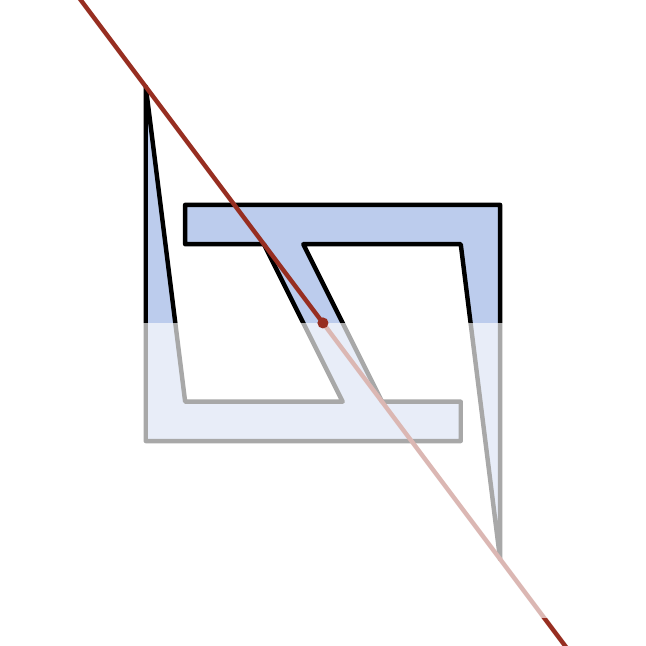
\begin{tikzpicture}[x=-0.5cm,y=0.5cm]
		\path (19.5, 11) circle (7.5);
		
		\draw[line join=round,fill=blue!50,ultra thick] (15,5) -- (16,13) -- (20,13) -- (18,9) -- (16,9) -- (16,8) -- (24,8) -- (24,17) -- (23,9) -- (19,9) -- (21,13) -- (23,13) -- (23,14) -- (15,14) -- cycle;
%		\draw[red,ultra thick] (19.5, 11) -- (16,4);
		
		\draw[red,ultra thick, shorten >= -8cm] (19.5, 11) -- (24,17);
		\draw[red,ultra thick, shorten >= -8cm] (19.5, 11) -- (15,5);
		
		\fill[white,opacity=0.66] let
			\p1=(current bounding box.south west),
			\p2=(current bounding box.south east)
		in
		(\x1,11) -- (\x1,\y1) -- (\x2,\y2) -- (\x2,11) -- cycle;
		
		\fill[red] (19.5, 11) circle (2pt);
%		\draw[red,-stealth,ultra thick] (19.5,11) -- (23,18) arc (63.43494:70:7.82624cm);
	\end{tikzpicture}
\end{document}